%
% main.tex -- Paper zum Thema <verkehr>
%
% (c) 2020 Hochschule Rapperswil
%
\chapter{Thema\label{chapter:verkehr}}
\lhead{Thema}
\begin{refsection}
\chapterauthor{Hans Muster}

Ein paar Hinweise für die korrekte Formatierung des Textes
\begin{itemize}
\item
Absätze werden gebildet, indem man eine Leerzeile einfügt.
Die Verwendung von \verb+\\+ ist nur in Tabellen und Arrays gestattet.
\item
Die explizite Platzierung von Bildern ist nicht erlaubt, entsprechende
Optionen werden gelöscht. 
Verwenden Sie Labels und Verweise, um auf Bilder hinzuweisen.
\item
Beginnen Sie jeden Satz auf einer neuen Zeile. 
Damit ermöglichen Sie dem Versionsverwaltungssysteme, Änderungen
in verschiedenen Sätzen von verschiedenen Autoren ohne Konflikt 
anzuwenden.
\item 
Bilden Sie auch für Formeln kurze Zeilen, einerseits der besseren
Übersicht wegen, aber auch um GIT die Arbeit zu erleichtern.
\end{itemize}

\section{Einführung}
\label{section:verkehr/einfuehrung}

\subsection{Verkehrsnetze}
Das Verkehrsnetz besteht aus allen Anlagen, auf oder unter der Erdoberfläche, auf denen eine räumliche Fortbewegung von Personen oder auch Gütern stattfindet. Verkehrsnetze sind ein Bestandteil der Verkehrsinfrastruktur, die auf topografischen Karten festgehalten werden. Sie umfassen den Schienenverkehr, alle Strassen und Wege, wie auch Flugplätze und alle dazugehörigen Bauwerke.
Aus verkehrsgeografischer Sicht besteht das Verkehrsnetz aus Kanten, Knotenpunkten und dem Hinterland. Die Knotenpunkte werden auch hier durch die Kanten verbunden, die den Verkehrsstrom aufnehmen, wobei das Hinterland durch einzelne Knoten versorgt wird. Die Aufteilung in Kanten und Knotenpunkte ermöglicht eine Vereinfachung komplexer Verkehrsnetze, damit sie mittels der Graphentheorie untersucht werden können.
Grundsätzlich können kurze Wege zwischen den Knotenpunkten das Ziel beim Aufbau eines Verkehrsnetzes sein. Es kann aber auch versucht werden, die Bau- und Unterhaltskosten des Verkehrsnetzes in einem gewissen Rahmen zu halten. Aus diesen Vorgaben ergibt sich dann, je nach dem was gewünscht wird, eine grob- oder feinmaschige Struktur des Netzes.
Ziel ist aber ein möglichst wirtschaftliches und optimales Verkehrsnetz.

\subsection{Suchalgorithmen}

\subsubsection{Dijkstra-Algorithmus}
Der Algorithmus von Dijkstra ist benannt nach seinem Erfinder dem Mathematik- und Infomratikprofessor Edsger Dijkstra. Den Algorithmus hat er im Jahr 1959 erfunden.
Der Algorithmus von Dijkstra ist ein Greedy-Algorithmus (gieriger Algorithmus), der schrittweise einen Folgezustand auswählt, damit beim Zeitpunkt der Wahl der grösste Gewinn bzw. das beste Ergebnis erzielt werden kann.
Trotz der Schnelligkeit der Greedy-Algorithmen, können viele Probleme nicht optimal gelöst werden.
Vereinfacht wird beim Dijkstra-Algorithmus, ausgehend von einem Startknoten so lange dem kürzesten Pfad gefolgt, bis der Zielknoten erreicht wird. Dabei muss für jeden besuchten Knoten die Kostenfunktion als auch der Pfad dahin (vorheriger Knoten) gespeichert werden.
Dadurch wird hingegen garantiert, dass, wenn der Zielknoten erreicht wird, auch der kürzeste Pfad gefunden wurde.
Grundlegende Voraussetzung für den Dijkstra-Algorithmus ist die strikte Positivität der Kantengewichte. Andernfalls würde ein wiederholtes Ablaufen einer Kante mit negativem Gewicht zu einer stetigen Reduktion der Kostenfunktion führen, was zu einer unendlichen Schlaufe führen würde.

Gegeben sei ein Netzwerk mit $n$ Knoten und dem Startknoten $a$.
Alle Kanten sind mit $k(i, j)$ bewertet.
Gesucht wird der kürzeste Pfad zwischen dem Startknoten und allen übrigen Knoten im Netz.
$D(i)$ ist die kürzeste Distanz vom Startknoten $a$ zum Knoten $i, V(i)$ ist der unmittelbare Vorgängerknoten vom Knoten $i$ auf dem kürzesten Weg vom Startknoten $a$ zum Konten $i$ und die Menge $M$ ist die Menge einer bestimmten Auswahl an Knoten.

Dabei gilt
\begin{equation}M={a}\end{equation}
\begin{equation}D(a)=0\end{equation} wobei
\begin{equation}D(i)=\infty\end{equation} und
\begin{equation}i \neq a \end{equation}
Ausserdem gilt \begin{equation}V(i)=(-) \text{für alle Knoten $i$}\end{equation}\\

%THEORIE...
Iteration

1. Auswahl eines Knotens \begin{equation} K\in M \text{mit} D(K)=D(i);i\in M\end{equation}

2. Für alle Nachfolger $N(j)$ vom Knoten $K$ gilt:
\begin{equation}D(K) + k_Kj < D(j)\end{equation} dann wird \begin{equation}D(j) = D(K) + k_Kj, V(j) = K\end{equation} gesetzt und somit wird der Knoten $j$ in die Menge $M$ aufgenommen.

3. Der ausgewählte Knoten \begin{equation}K\in M\text{wird aus der Menge herausgelöscht}\end{equation}\\
Diese drei Schritte werden so lange wiederholt bis gilt
\begin{equation}M=\{\}\end{equation}

\subsubsection{A*-Algorithmus}
Suchalgorithmen werden nach einfachen (uninformierte) und heuristischen (informierten) Algorithmen unterschieden. Während einfache Algorithmen den Suchraum intuitiv durchsuchen, beziehen heuristische Algorithmen Wissen über den Suchraum mit ein.
Der A*-Algorithmus geht auf seine Erfinder Peter Hart, Nils Nilsson und Bertram Raphael zurück, die den Algorithmus erstmals im Jahr 1968 beschrieben.
Der A*-Algorithmus ist ein heuristischer Suchalgorithmus, der den kürzesten Pfad zwischen zwei Knoten in einem Graphen mit positiven Kantengewichten berechnet.
Im Gegensatz zu einfachen Suchalgorithmen, wird beim A*-Algorithmus eine Schätzfunktion, die sogenannte Heuristik, verwendet. Dies ermöglicht ein zielgerichtetes Suchen und gleichzeitig wird die Laufzeit verringert.
Ausserdem findet der A*-Algorithmus immer eine optimale Lösung, sofern eine vorhanden ist.
Der A*-Algorithmus wird als Verallgemeinerung gehandhabt und gilt als Erweiterung des Dijkstra-Algorithmus.

\subsubsection{Anwendung A*-Algorithmus}
Wie oben erwähnt basiert der A*-Algorithmus auf dem Shortest-Path-Algorithmus von Dijkstra. Gemäss dem Algorihtmus von Dijkstra werden von einem Startknoten aus die jeweiligen Nachbarknoten, die Nachbarknoten der Nachbarknoten usw. verarbeitet. Die Kantengewichte werden dabei aufsummiert und die Priorität wird auf die Kante gelegt, die das geringste Gewicht aufweist. Mit diesem Verfahren wird sichergestellt, dass die erste gefundene Lösung auch die optimalste Lösung darstellt.\\

Die Kantengewichte werden für jeden Knoten in Form einer Funktion dargestellt
\begin{equation}f(n)=g(n)\end{equation} mit
\begin{equation}g(n)=\text{Summe aller Kantengewichte vom Startknoten bis n}\end{equation}\\
Der A*-Algorithmus erweitert die Vorgehensweise des Algorithmus von Dijkstra um die Heuristik $h(n)$, die für jeden Knoten $n$ die geschätzte Entfernung zum Zielknoten beschreibt.
Somit gilt:
\begin{equation}f(n)=g(n)+h(n)\end{equation}\\
Wie auch der Algorithmus von Dijkstra findet der A*-Algorithmus die optimalste Lösung.

\subsubsection{Floyd-Warshall-Algorithmus}
Der Floyd-Warshall-Algorithmus, auch Tripel-Algorithmus genannt, wurde erstmals im Jahr 1962 von seinen Namensgebern Robert Floyd und Stephen Warshall vorgestellt.
Der Floyd-Warshall-Algorithmus sucht kürzeste Wege innerhalb eines Graphen. Er ermittelt aber nicht nur die Distanz zwischen zwei Knoten, sondern berechnet die kürzesten Wege zwischen allen Knotenpaaren eines gewichteten Graphen. Somit werden die kürzesten , beziehungsweise die optimalsten Wege zwischen allen Paaren von Knoten berechnet. Der Floyd-Warhshall-Algrithmus kann ausserdem mit negativen Kantengewichten umgehen, sofern der Graph aber keinen negativen Kreis (Zyklus) aufweist. Ist dies der Fall, führt der Algorithmus zu einem falschen Ergebnis.
Ein Kreis (Zyklus) in einem Graphen ist ein Weg, bei dem Start- und Endpunkt den gleichen Knoten aufweisen. Dieser wird negativ, wenn die Summe der gewichteten Kanten kleiner als Null wird.\\
Der Floyd-Warshall-Algorithmus besteht grundsätzlich aus Floyd's Berechnung der kürzesten Distanzen zwischen zwei Knoten und Warshall's Konstruktion der kürzesten Wege. Werden diese beiden Teilgebiete zusammengefügt, ergibt sich der Floyd-Warshall-Algorithmus.

\subsubsection{Anwendung Floyd-Warshall-Algorithmus}

Wie oben erwähnt, besteht der Floyd-Warshall-Algorithmus aus dem Teil von Floyd zur Berechnung der kürzesten Pfade und dem Teil von Warshall zur Konstruktion der kürzesten Pfade.

%THEORIE...
Als erstes wird eine Gewichtsmatrix $W$ mit den Matrixeinträgen $W[i, j]$ erstellt.
Der Algorithmus berechnet danach in einer Hauptschleife alle Knoten $k$ von 1 bis $n$.
Dabei versucht er in jeder Iteration alle Wege von $i$ nach $j$ durch die Wege $(i, k)$ und $(k, j)$ zu verbessern.
Falls dieser mögliche Umweg zu einer Verbesserung führt, wird der Algorithmus aktualisiert.

Die aktuelle Gewichtung der Pfade wird mit
\begin{equation}d[i, j]=min[d[i,j], d[i,k] + d[k,i]]\end{equation}
ermittelt.

\subsubsection{Euklidische Heuristik}
Bei Verkehrsnetzen ist die euklidische Distanz eine gängige und zuverlässige Heurstik. Dabei wird zu den effektiven Reisekosten zum aktuellen Knoten die euklidische Distanz bis zum Zielknoten hinzuaddiert. Dadurch wird die Kostenfunktion konsequent nie überschätzt. Dies stellt eine Voraussetzung an eine zulässige Heuristik dar.
Was bei einem physischen Verkehrsnetz einfach zu bewältigen ist, da Koordinaten von Verkehrsnetzen zur Berechnung der Distanz verwendet werden können, ist bei virtuellen Netzwerken (z.B. Servernetzen) entweder nicht möglich, oder nicht relevant.

\subsection{PageRank-Algorithmus}
Der PageRank-Algorithmus wurde von den Gründern von Google, Larry Page und Sergey Brin im Jahr 1996 entwickelt und zum Patent angemeldet. Zwei Jahre später gründeten sie ihr Unternehmen Google Inc..
Beim PageRank-Algorithmus handelt es sich um den Algorithmus von Google, aus dem die Google-Matrix abgeleitet wird.
Die Google-Matrix ist eine immens grosse Matrix mit Millionen Zeilen und Spalten, die für die schnelle und vor allem exakte Bestimmung der PageRanks (Gewichtung) eine grosse Bedeutung hat.
Der PageRank-Algorithmus analysiert und gewichtet beispielsweise die Verlinkungsstruktur verschiedener Websites des World Wide Web anhand ihrer Struktur.
Der PageRank wird umso höher, je mehr hochwertige Links auf eine Webseite verweisen und je höher die Gewichtung einer Webseite ist, desto grösser ist der Effekt.\\
Dabei handelt es sich um einen iterativen Prozess. Ausgegangen wird von der Adjazenz-Matrix $A$, für welche gilt.

%THEORIE...
Grundsätzlich setzt sich der PageRank Algorithmus mit der Fragestellung auseinander, wie eine Suchmaschine wie Google Suchresultate bewertet und somit sortieren soll. Öfters aufgerufene Resultate sollen schliesslich höher gewichtet werden. Dabei wird angenommen, dass eine Website populärer ist, je mehr andere Websites darauf verweisen.

\begin{equation}
A_{i,j}=\left\{ \begin{matrix}
1 & \text{Kante von $j$ nach $i$} \\ 0 & \text{keine Kante von $j$ nach $i$}
\end{matrix}
 \right.
\label{verkehr:Adja}
\end{equation}


Für ungerichtete Graphen mit $n$ Knoten gilt \begin{equation}A_{i,j}=A_{j,i}\end{equation} und weiter \begin{equation}A_{i,i}=0\quad\forall i\in \left\{1...n\right\}\end{equation}
Beim PageRank-Algorithmus wird eine abgewandelte Form der Adjazenz-Matrix verwendet.
Dabei werden die Matrix-Einträge spaltenweise durch die jeweilige Spaltensumme geteilt.
\begin{equation} P_{i,j}=\frac{A_{i,j}}{\sum_{i=1}^{n}A_{i,j}} \end{equation}
Anschliessend multipliziert man diese Matrix $P$ mit einem Spaltenvektor $\Vec{r_0}$ mit $n$ Einträgen, für welchen gilt:
\begin{equation} \Vec{r_0}(i) = \frac{1}{n} \quad\forall i\in \left\{1...n\right\} \end{equation}
Dieser Vektor stellt ein neutrales Ranking dar. Alle Knoten werden gleich gewichtet.
Dadurch erhält man wiederum einen $n$-zeiligen Spaltenvektor $\Vec{r_1}$, der das "erste" Ranking darstellt. Durch Multiplikation der ursprünglichen Matrix $P$ mit dem 1. Ranking-Vektor $\Vec{r_1}$ wird auf Basis des ersten Rankings ein zweites erstellt.
\begin{equation} \Vec{r_2} = P\cdot\Vec{r_1} = P\cdot(P\cdot\Vec{r_0}) = P^2\cdot\Vec{r_0}\end{equation}
somit
\begin{equation} \Vec{r_i} = P^i\cdot\Vec{r_0}\end{equation}
Der Vektor $\Vec{r_i}$ konvergiert zu einem Eigenvektor von $P$ und stellt das abschliessende Ranking dar.

\section{Versuchsreihe}
\label{section:verkehr/versuchsreihe}

Um zwei der vorgestellten Suchalgorithmen zu vergleichen, wurden zwei Versuchsreihen erstellt. Dazu wurden in einem ersten Schritt zufällige Netzwerke generiert und anschliessend der Dijkstra- und der A*-Algorithmus auf das Netzwerk angewandt.
Dieser Vorgang wurde für die zufällig generierten Netzwerke mit einer Knotenzahl von 10, 20 50, 100, 200, 500 und 1000 je zehnmal wiederholt.
Die Anzahl der Knoten im abgesuchten Netzwerk wirkt sich direkt auf die Rechenzeit aus. Der \emph{Dijkstra}-Algorithmus weist eine Zeitkomplexität von $\mathcal{O}(E\log{}V)$ auf, wobei $E$ die Menge der Kanten (engl. \emph{edges}) und $V$ die Menge der Knoten (engl. \emph{vertices}) des Graphen $G$ darstellt.
Für den A*-Algorithmus ist die Zeitkomplexität einerseits abhängig von der verwendeten Heuristik, andererseits aber auch vom vorliegenden Netzwerk selbst. Aus diesem Grund lässt sich keine defintive Angabe zur Zeitkomplexität machen.

Die beiden Versuchsreihen unterscheiden sich zudem dahingehend, dass der Start- und Zielknoten bei der ersten Versuchsreihe im Netzwerk diametral gegenüber liegen. Dadurch gehen viele Knoten verloren, welcher \emph{Dijkstra} als uninformierter Suchalgorithmus absuchen würde. In der zweiten Veruschsreihe werden hingegen Start- un Zielpunkt zufällig im Netzwerk ausgewählt. Es wird deshalb erwartet, dass die Unterschiede in der Rechenzeit der beiden Algorithmen in der zweiten Versuchsreihe deutlich ausgeprägter sind.

\subsection{Einfluss der Knotenzahl auf die Rechenzeit}
\label{verkehr:Knotenzahl}

\begin{figure}
\centering
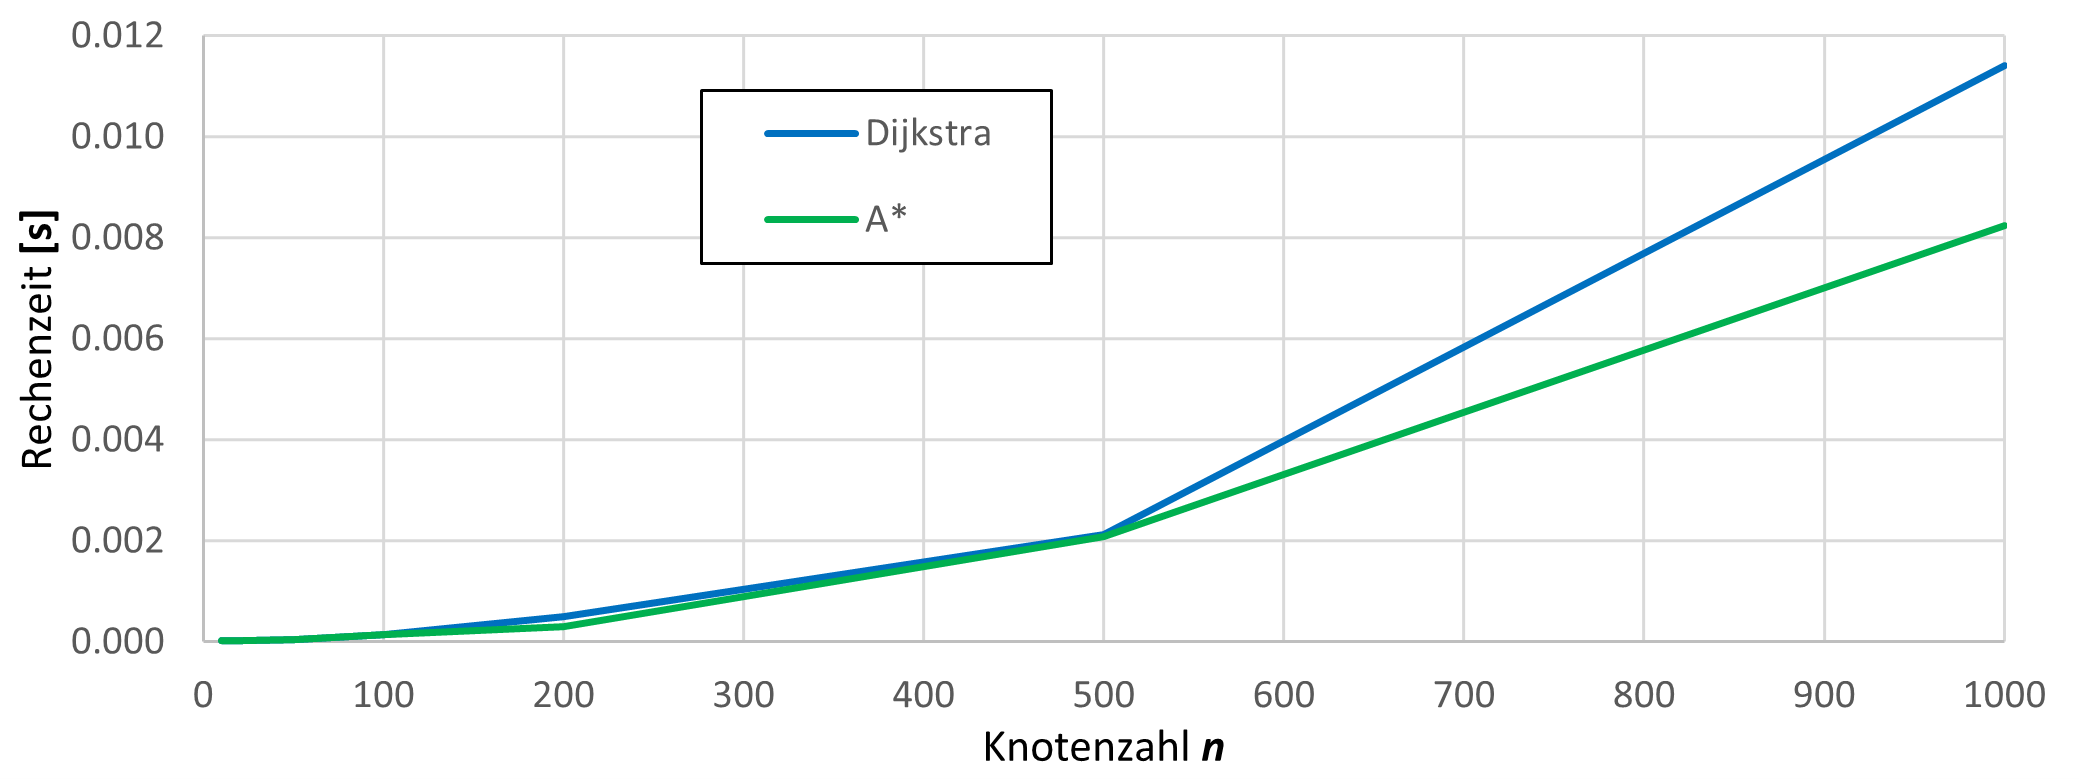
\includegraphics[width=12cm]{papers/verkehr/figures/chart_Vr1.png}

\caption{Gemessene Rechenzeiten der ersten Versuchsreihe in Abhängigkeit der Knotenzahl.}
\label{verkehr:Vr1}
\end{figure}

In \ref{verkehr:Vr1} ist ersichtlich, dass der Unterschied in der Rechenzeit zwischen Dijkstra und A* erst ab einer Knotenzahl von ca. $n=500$ merklich ansteigt. Dieses etwas überraschende Resultat ist darauf zurückzuführen, dass bei steigender Knotenzahl die Abweichung des effektiven kürzesten Pfades von der Distanz der Luftlinie abnimmt.
Die Effektivität von \emph{A*} mit euklidischer Heuristik ist wiederum grösser, wenn die Abweichung des kürzesten Pfads von der Luftlinie minimal ist.
Abbildung \ref{verkehr:pathDifference} illustriert dies, wobei die relative Abweichung erstaunlicherweise bei einer Knotenzahl von $n=100$ maximal ist und nach $n=500$ nur noch marginal abnimmt.

\begin{figure}
\centering
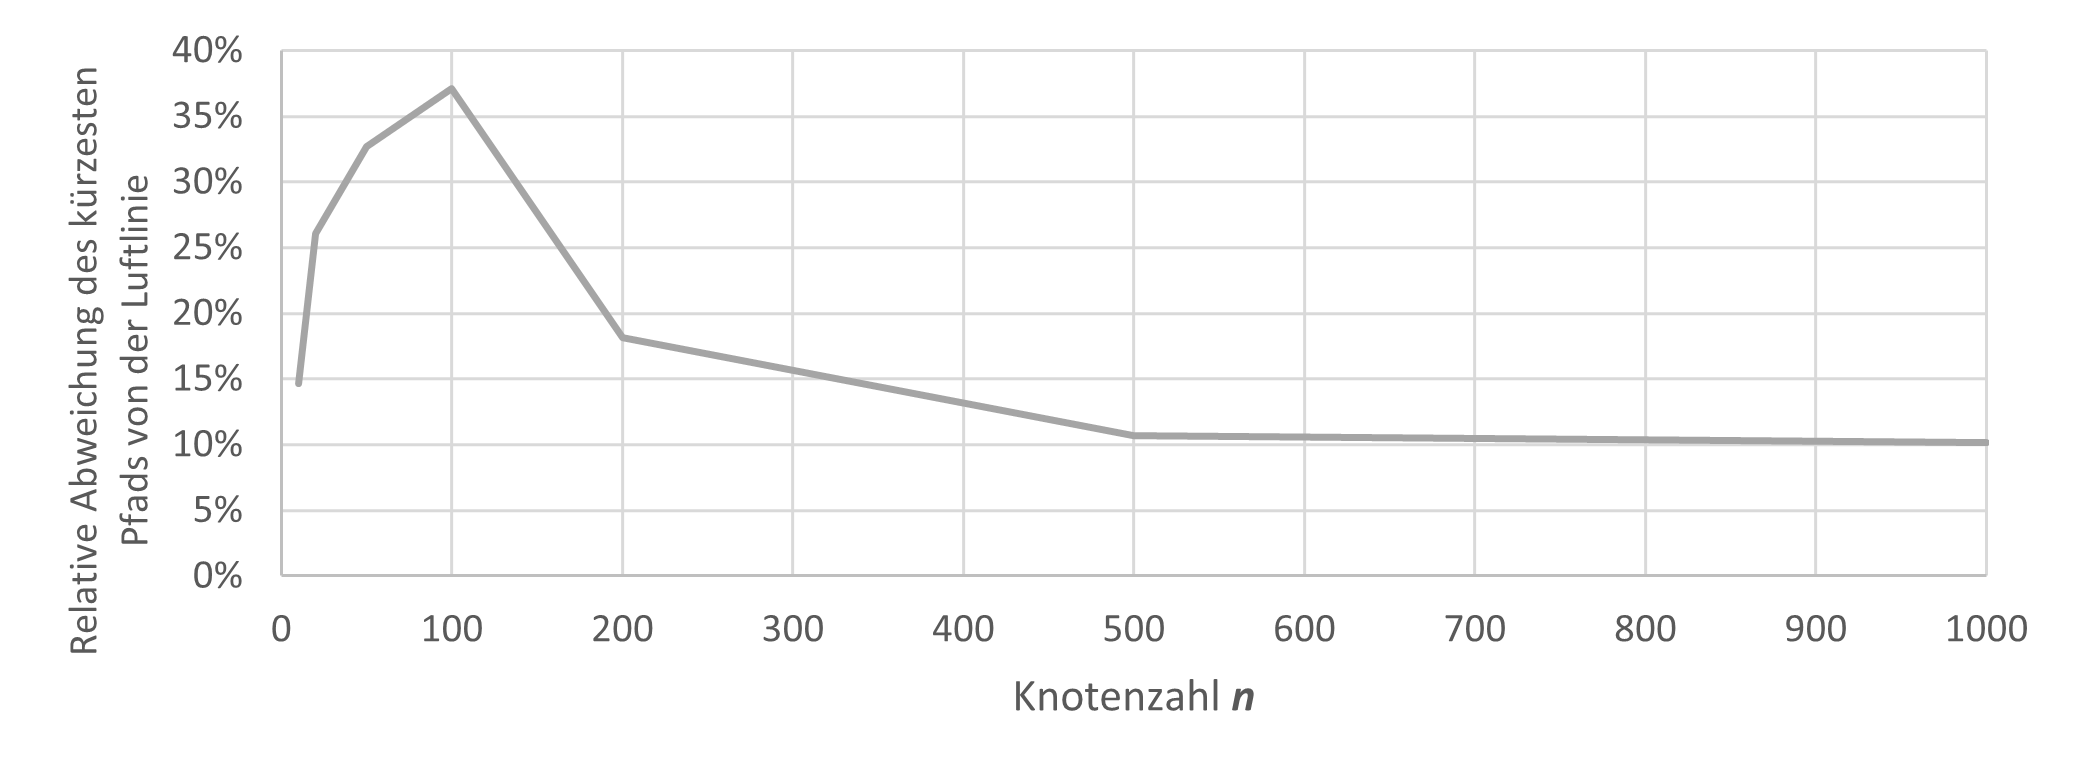
\includegraphics[width=12cm]{papers/verkehr/figures/chart_pathDiff.png}

\caption{Relative Abweichung des kürzesten Pfads von der Luftlinie.}
\label{verkehr:pathDifference}
\end{figure}


\subsection{Einfluss der Position der Start- und Zielknoten auf die Rechenzeit}

\begin{figure}
\centering
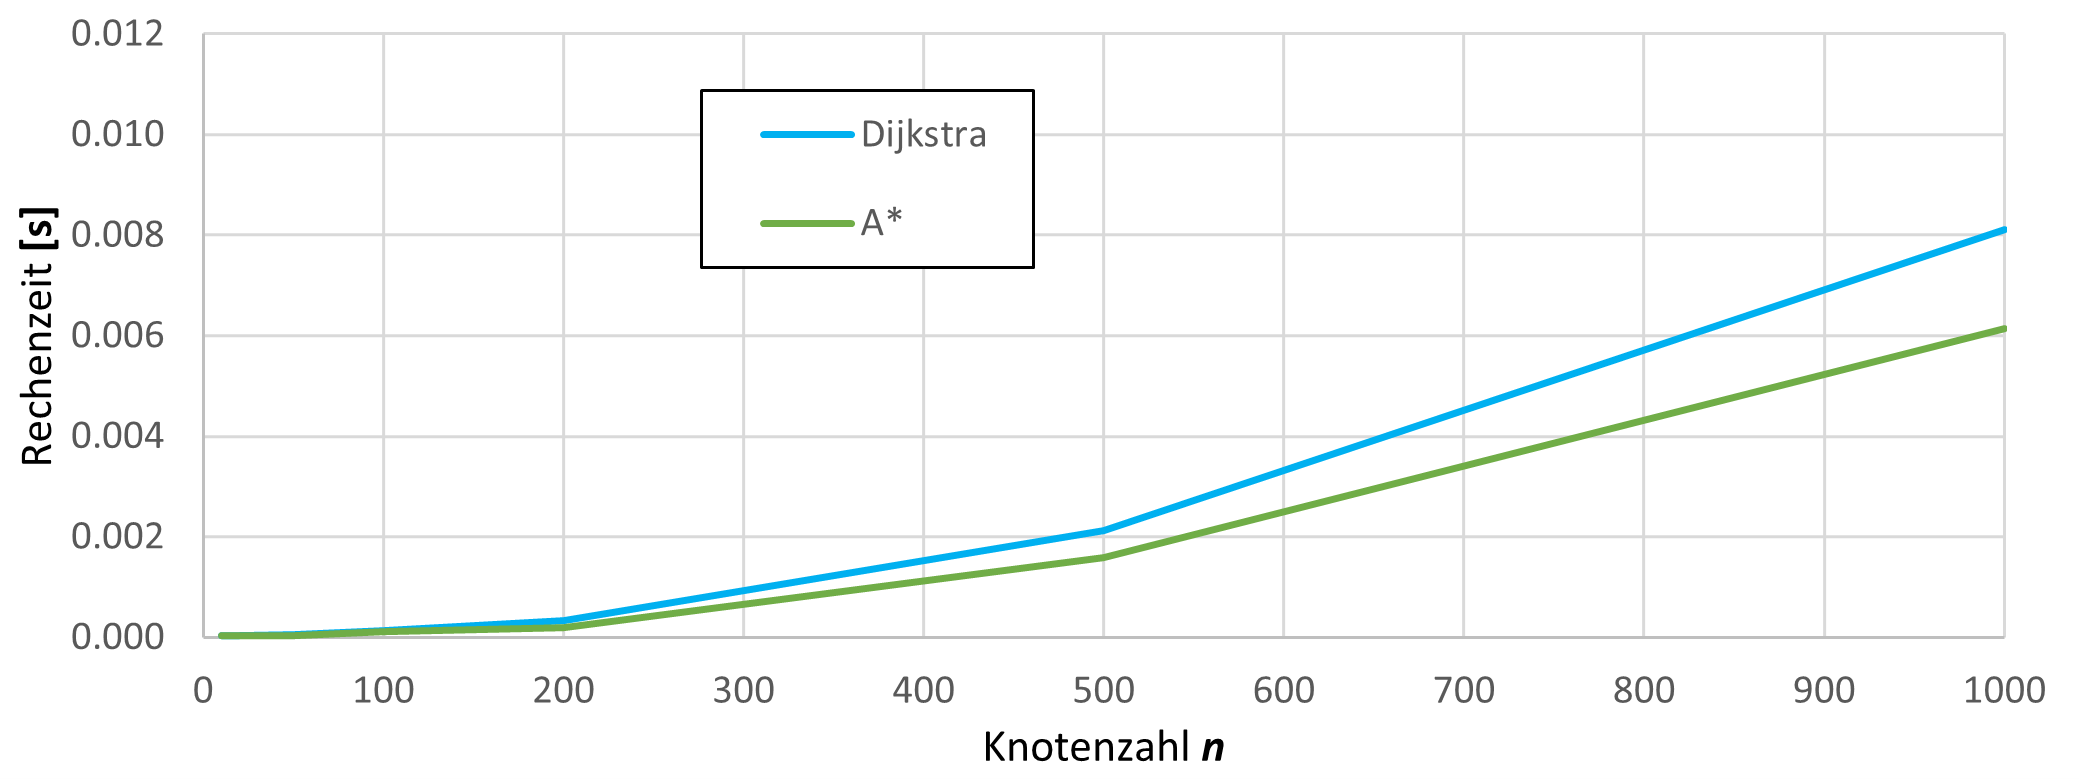
\includegraphics[width=12cm]{papers/verkehr/figures/chart_Vr2.png}
\caption{Gemessene Rechenzeiten der zweiten Versuchsreihe in Abhängigkeit der Knotenzahl.}
\label{verkehr:Vr2}
\end{figure}

Zum Vergleich der Resultate in Abschnitt \ref{verkehr:Knotenzahl} zeigt Abbildung \ref{verkehr:Vr2} die Rechenzeiten der zweiten Versuchsreihe, in welcher die Start- und Zielknoten zufällig im Netzwerk ausgewählt wurden. Einerseits ist eine reduzierte durchschnittliche Rechenzeit festzustellen, was daran liegt, dass die zufällige Wahl der Knoten dazu führt, dass diese tendenziell weniger weit auseinander liegen.
Des weiteren ist festzustellen, dass sich die Unterschiede der Rechenzeiten zwischen Dijkstra und A* deutlich früher abzeichnen. Dieses Phänomen lässt sich leicht durch die zielgerichtete Suche des A*-Algorithmus erklären.

\begin{figure}
\centering
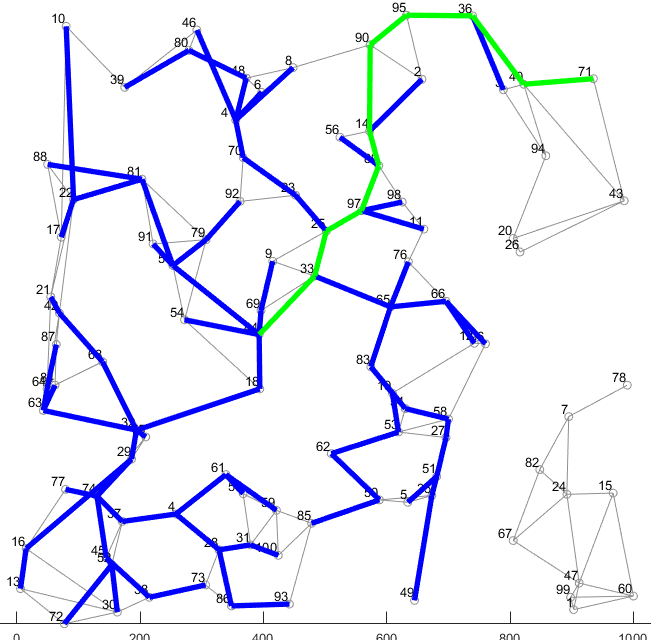
\includegraphics[width=6cm]{papers/verkehr/figures/network_dij.png}\qquad
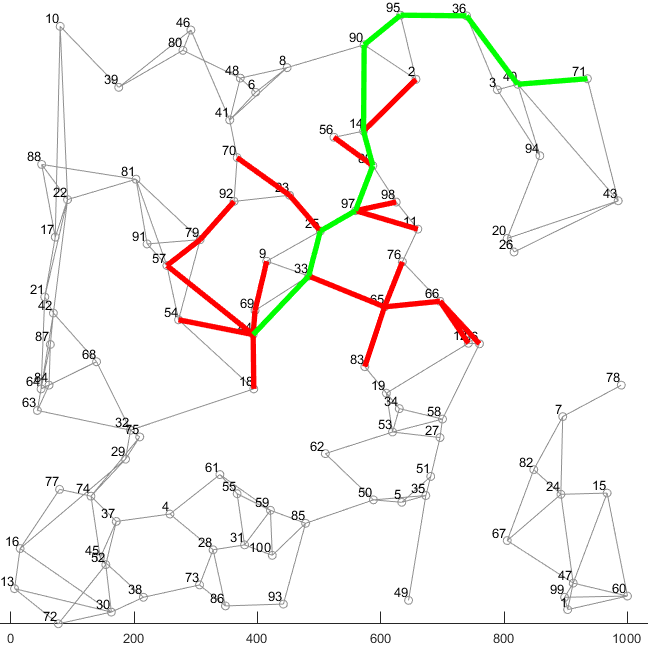
\includegraphics[width=6cm]{papers/verkehr/figures/network_aStar.png}
\caption{Suchpfad in grün mit \emph{Dijkstra} (links), und \emph{A*} (rechts). Besuchte Knoten sind in blau, resp. rot markiert.}
\label{verkehr:Comparison}
\end{figure}

In Abbildung \ref{verkehr:Comparison} ist ersichtlich, dass bei einem im Netzwerk liegenden Startknoten die zielgerichtete Suche von \emph{A*} deutlich ausgeprägter zum Zuge kommt, als wenn dieser am Rand des Netzwerks liegen würde.

\section{Ausblick}
\subsection{Optimierungsprobleme bei Graphen}
Das Finden eines kürzesten Pfades, sprich die Minimierung der Summe der Kantengewichte, ist nur eines der Optimierungsprobleme, die sich im Bereich von Graphen aufstellen lassen. Verschiedene, ähnliche Problemstellungen lassen sich teilweise mit denselben Algorithmen lösen.

Im Bereich vom Computernetzwerken könnte zum Beispiel die Minimierung der Knotenzahl zur Datenübbertragung von Interesse sein. Dabei lässt sich dieses Problem einfach dadurch lösen, dass dem Dijkstra- oder dem A*-Algorithmus anstelle der gewichteten Adjazenz-Matrix (mit Kantengewichten als Einträgen) die ungewichtet Adjazenz-Matrix als Argument übergeben wird. Der gefundene kürzeste Pfad enstpricht der Anzahl benutzter Kanten, bzw. der Anzahl besuchter Knoten.  

\subsection{Wahl der Heuristik}
Ein grundlegendes Problem bei der Anwendung des A* oder ähnlicher informierter Suchalgorithmen ist die Wahl der Heurstik. Bei einem physischen Verkehrsnetz kann bspw. die euklidische Distanz problems ermittelt werde. Bei einem regionalen Netzwerk ist die Annahme eines orthogonalen X-Y-Koordinatenetzes absolut ausreichend. Dies gilt z.B. auch für das Vernessungsnetz der Schweiz\footnote{Die aktuelle Schweizer Referenzsystem LV95 benutzt ein E/N-Koordinatennetz, wobei aufgrund zunehmender Abweichung vom Referenzellipsoid bei grosser Entfernung vom Nullpunkt ein Korrekturfaktor für die Höhe angebracht werden muss.} Bei überregionalen Netzwerken (Beispiel: Flugverbindungen) ist hingegen eine Berechnung im dreidimensionalen Raum, oder vereinfacht als Projektion auf das Geoid notwendig. Anonsten ist der Ablauf bei der Ausführung des Algorithmus allerdings identisch.
In nicht-physischen Netzwerken stellt sich jedoch eine zweite Problematik. Da eine physische Distanz entweder nicht ermittelt werden kann, oder aber nicht ausschlaggebend ist, sind andere Netzwerk-Eigenschaften zur Beurteilung beizuziehen. Die Zuverlässigkeit ist dabei aber in den meisten Fällen nicht vergleichbar hoch, wie bei der euklidischen Heuristik. Oftmals werden deshalb bei derartigen Problem auch Algorithmen angewendet, die eine deutlich optimierte Zeitkomplexität aufweisen, dafür aber nicht mit Sicherheit den effizienstesten Pfad finden.


\printbibliography[heading=subbibliography]
\end{refsection}
